\subsection{Infinite plate with a circular hole}
\paragraph{}
In this example, an infinite plate with a traction free hole under uniaxial tension $(\sigma = 1 N/m^2 )$
along x-axis (see fig.~\ref{iso_fig:circular_hole_geo_bc}) is considered.

    \begin{figure}[h!]
        \centering
        \scalebox{0.75}{
            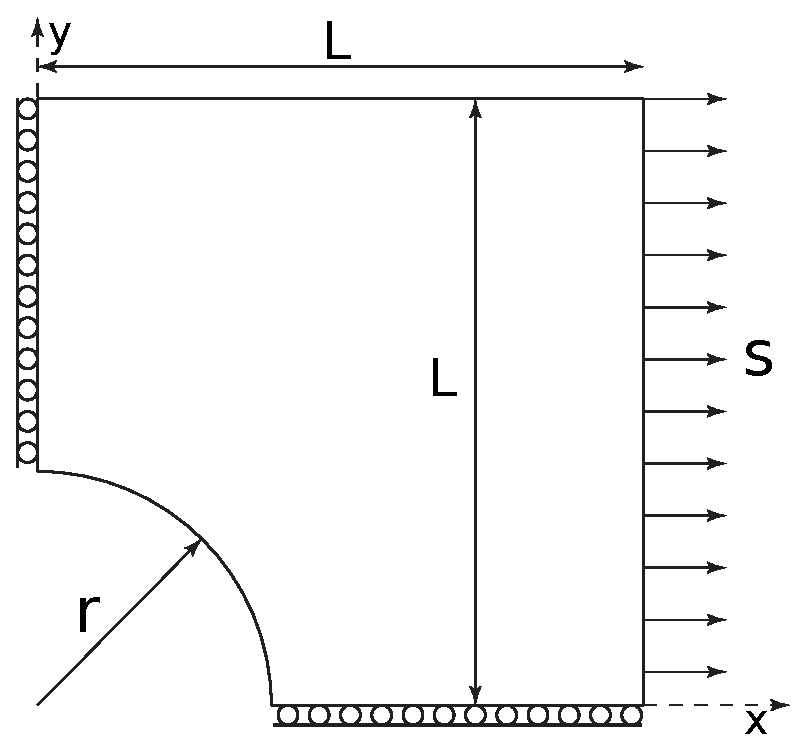
\includegraphics{isogeometric_sbfem/images/circular_hole_geo_bc.eps}
        }
        \caption{ Infinite plate with a circular hole: geometry and boundary conditions}
        \label{qdt_fig:circular_hole_geo_bc}
    \end{figure}
    
The exact solution of the principal stresses in Cartesian coordinate $(r,\theta)$ is given by \cite{Sukumar2001} in eq.~\ref{iso_eq:ex_chole_stress_sol}.
